\subsection{Private chain}

The structure of the private block is shown in Figure \ref{fig:privateblocks}. The block consists of a public \textit{header} that the Educators relay to the Witnesses, and the private \textit{body} that remains in the educational institute until it receives a data disclosure request.

\begin{figure}[ht]
\centering
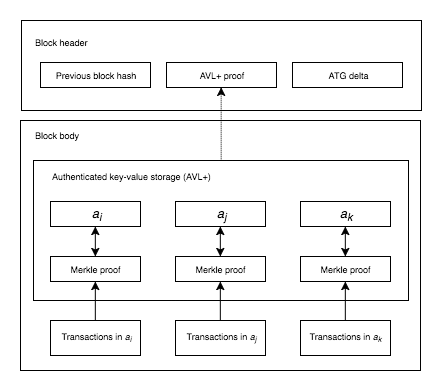
\includegraphics[width=0.8\textwidth]{private-blocks}
\caption{Private block structure}
\label{fig:privateblocks}
\end{figure}

During the educational process the Educators emit atomic \textit{private transactions}. These tansactions represent the modifications to the journal of academic achievements in a certain activity type (thus, making a transaction means appending the data to the journal of a particular course). The transactions can be of the following types:
\begin{itemize}
\item student enrolls in a course;
\item student gets an assignment;
\item student submits an assignment;
\item student gets a score for an assignment;
\item student gets a final score for the course.
\end{itemize}

Let us denote an $i$-th transaction belonging to a certain activity type $a_j$ as $T_{a_j}^i$. The Educators group the transactions that occured during the current block time slot according to the activity type, and construct Merkle trees \cite{merkle1989certified} for these journal modifications:
\begin{equation}
M_{a_j} = \MerkleTree(T_{a_j}^i)
\end{equation}

The Educator's private block body contains a dictionary of key-value pairs, where each key is the leaf in the activity type graph $a_j$, and the values are the Merkle roots of all the transactions that occurred in this leaf in the current block. Thus, the private block body is a mapping:
\begin{equation}
a_j \rightarrow \Root(M_{a_j})
\end{equation}

In order to make this mapping easily verifiable, we use a structure called the \textit{authenticated AVL+ tree} introduced in \cite{reyzin2016improving}. This structure is based on state-of-the-art research that enables for faster verification of the mapping and allows us to never disclose it: the Witnesses would not have to store the whole blockchain like Bitcoin or Ethereum nodes do. Rather, they would just have to check the private block headers in order to confirm that none of the private blocks were tampered with.

The private block header consists of the AVL+ proof along with the previous block hash and the information on the Activity Type Graph modifications (ATG delta). The \textit{ATG delta} part allows the Educators to inform the Witnesses and the Archivists of the modifications to the courses they teach.

After the end of the block time slot, an Educator signs the block header and submits it to the Witnesses so that the private transactions can be confirmed by the public chain. Thus, the private blocks form a publicly verifiable chain of events, grouped according to the activity type.
